The analysis strategy relies on the use of a binary classification algorithm to create regions of high \ttH purity.
A boosted decision tree (BDT) is chosen as the binary classification algorithm.
Deep neural networks (DNNs) were also explored; however, these were found to outperform BDTs only when a very high number of training examples are available (discussed in further detail in Sec.~\ref{sec:tth_dnns}).
The BDT-bkg algorithms are trained with the \textsc{xgboost}~\cite{xgboost} framework, using MC simulation of \ttH for the signal events and a combination of MC simulation and data-driven descriptions of the relevant background processes as background.
In order to avoid bias, the BDT-bkg algorithms are trained and optimized on completely separate samples from those used in the measurement of $\mu_{\ttH}$.
The various background processes are weighted according to their cross sections, while the weights of signal events are scaled such that the total number of signal events is equal to the total number of background events.
The signal weights are scaled in such a fashion to avoid issues in training related to imbalanced classes.
The features used in training the BDT-bkg algorithms are discussed in the following subsections. 

\subsection{High-Level Features} \label{sec:tth_hlf}
In order to effectively separate \ttH from the SM backgrounds, we construct a number of high-level physics variables which are expected to have discriminating power between the two.
The full list of features is shown in Table~\ref{tab:tth_hlf}.
Plots showing the distributions for both data and simulation for each input feature are shown in Appendix~\ref{app:hlf}.

\begin{table}[h] \scriptsize
\centering
\renewcommand{\arraystretch}{1.5}
\begin{tabular}{|c| c c c|}
\multicolumn{4}{c}{Input Features to BDTs} \\ \hline
Category & \multicolumn{3}{c|}{Features} \\ \hline
\multirow{3}{*}{Photon Kinematics} & $\gamma_1$ $p_T$/$m_{\gamma \gamma}$ & $\gamma_1$ $\eta$ & $\gamma_1$ Pixel Seed Veto \\
& $\gamma_2$ $p_T$/$m_{\gamma \gamma}$ & $\gamma_2$ $\eta$ & $\gamma_2$ Pixel Seed Veto \\
& Max $\gamma$ ID MVA & Min $\gamma$ ID MVA & \\ \hline
\multirow{7}{*}{Jet Kinematics} & Jet 1 $p_T$ & Jet 1 $\eta$ & Jet 1 b-tag score \\
& Jet 2 $p_T$ & Jet 2 $\eta$ & Jet 2 b-tag score \\
& Jet 3 $p_T$ & Jet 3 $\eta$ & Jet 3 b-tag score \\
& Jet 4 $p_T$ & Jet 4 $\eta$ & Jet 4 b-tag score \\
& Max b-tag score & 2nd max b-tag score & \\
& $N_{\text{jets}}$ & $H_T$ & \\ \hline
\multirow{2}{*}{DiPhoton Kinematics} & $p_T^{\gamma \gamma} / m_{\gamma \gamma}$ & $Y_{\gamma \gamma}$ & $|\cos (\Delta \phi)_{\gamma \gamma}|$ \\
& $\Delta R_{\gamma \gamma}$ & $|\cos(\text{helicity angle} (\theta))|$ & \\ \hline
Lepton Kinematics & lepton $p_T$ & lepton $\eta$ & $N_{\text{leptons (tight ID)}}$ \\ \hline
\multirow{1}{*}{Event-level Kinematics} & $E_T^{\text{miss}}$ & & \\ \hline
\end{tabular}
\caption{High level features used in training BDTs. The fourth jet kinematics are given as input features only to the BDT-bkg in the hadronic channel, while the lepton kinematics are given as input features only to the BDT-bkg in the leptonic channel.} 
\label{tab:tth_hlf}
\end{table}

The physics motivations for the inclusion of each feature are enumerated below:
\begin{enumerate}
    \item Photon Kinematics
    \begin{itemize}
        \item Photon \pT divided by \mgg: prompt photons tend to have higher transverse momentum than fake photons from hadronic jets. The photon \pT is normalized by \mgg to prevent the BDT from learning \mH.
        \item Photon $\eta$: prompt photons tend have smaller $|\eta|$ than fake photons.
        \item Photon pixel seed veto: \ttplusX events often have one or more electrons from leptonically decaying \PW bosons which are identified as photons at reco-level. The pixel seed veto helps identify these events.
        \item Photon ID MVA: the primary means of separating between prompt and fake photons. Described in further detail in Sec.~\ref{sec:evt_photon_idmva}.
    \end{itemize}
    \item Jet Kinematics
    \begin{itemize}
        \item Jet \pT: jets from \ttH events tend to have higher transverse momentum than those from background processes (both multi-jet + X and \ttplusX), as the \ttb system recoils against the Higgs.
        \item Jet $\eta$: jets from \ttH tend to be more central than those from multi-jet + X events.
        \item Jet b-tag scores: jets from \ttH have higher b-tag scores than those from non-\ttb backgrounds, as two b-jets are expected 2 from the \ttb decay. 
        \item Number of jets: we expect at least 6 (4) jets in a \ttH event in the Hadronic (Leptonic) channel.
        \item $H_{\text{T}}$: \ttH events tend to have higher values of $H_{\text{T}}$, due to the fact that we expect higher $p_T$ of individual jets as well as more total jets in the event.
    \end{itemize}
    \item DiPhoton Kinematics
    \begin{itemize}
        \item DiPhoton \pT divided by \mgg: the recoil of the Higgs against the \ttb system results in higher expected values for the diphoton momentum. The DiPhoton \pT is normalized by \mgg to prevent the BDT from learning \mH.
        \item DiPhoton $Y$: the DiPhoton rapidity is expected to be closer to zero for \ttH events.
        \item DiPhoton $\Delta R$: the angle between the two photons is expected to be smaller for \ttH events due to the fact that the Higgs tends to be boosted from recoil against the \ttb system.
        \item Helicity angle ($\theta$): defined by boosting to the rest frame of the DiPhoton pair and calculating the angle between the photons in that frame. Since the SM Higgs is a scalar, we expect a uniform distribution in $\cos(\theta)$ for \ttH (at generator-level), while backgrounds may peak closer to 1.
        \item $\cos (\Delta \phi)$ of DiPhoton pair: similar argument to above.
    \end{itemize}
    \item Lepton Kinematics
    \begin{itemize}
        \item Lepton \pT: prompt leptons tend to have higher \pT than fake leptons from hadronic jets.
        \item Lepton $|\eta|$: prompt leptons tend to be more central than fake leptons.
        \item Number of leptons passing tight ID: again, helpful in discriminating between prompt and fake leptons. The preselection requires that leptons pass medium ID, the number of leptons passing tight ID is given as an input to the BDT.
    \end{itemize}
    \item Event-level Kinematics
    \begin{itemize}
        \item \met: in the Leptonic channel, we expect nonzero \met in \ttb events due to the neutrino from the $\PW\to l\nu$ decay, while no \met is expected for multi-jet + X events. In the Hadronic channel, this may also be useful in identifying leptonically decaying \ttH events in which the lepton is not reconstructed.
    \end{itemize}
\end{enumerate}

\subsection{Deep Neural Networks for \dipho and \ttgg Backgrounds} \label{sec:tth_dnns}
The dominant SM backgrounds in regions of high \ttH purity (i.e. similar to the signal regions) are: \dipho and \ttgg in the hadronic channel, and \ttgg in the leptonic channel.
To further reduce these backgrounds, additional methods and variables designed to specifically target these backgrounds were explored.
Among the most successful of these methods were deep neural networks (DNNs) trained to reject these backgrounds specifically.
Another notable susccessful tool is the top tagger BDT, discussed in Sec.~\ref{sec:tth_top_tagger_bdt}.

The DNNs exploit low-level information in each event which is lost in the process of summarizing the event in terms of the high-level features described in Sec.~\ref{sec:tth_hlf}.
An example of such low-level information is the azimuthal angle $\phi$ of the reconstructed jets and leptons.
Any physics process should obey azimuthal symmetry in the CMS detector -- any value of $\phi$ is equally likely for any physics object from any physics process.
For this reason, the $\phi$ value of a given jet or lepton on its own provides no means to discriminate between \ttH and other SM backgrounds.
However, the $\phi$ value of a jet or lepton may provide discriminatory power when considered in the context of the rest of the event: angles between jets and leptons likely have different distributions in \ttH events and SM background events.
Providing this type of low-level input to a BDT would be of limited use, as making a splitting on the $\phi$ value of a jet or lepton is not useful on its own.
Deep neural networks were then explored as an algorithm which could potentially make better use of such low-level features.

\subsubsection{Training Features}
The high-level features described in Sec.~\ref{sec:tth_hlf} do not retain the full information of the original event.
To provide a more complete description of each event, the four-vectors of the leading jets and leptons (``physics objects'') are given as inputs to the DNNs.
The four-vector includes the physics object's \pT, $\eta$, $\phi$, and total energy ($E$).
In addition to the four-vectors, four jet flavor scores and lepton ID flags, indicating whether a given lepton is a muon or electron are provided for each physics object.
In total, for up to the leading eight (six) jets in each event and the leading zero (two) leptons in each event in the Hadronic (Leptonic) channel, the following nine features are provided for each physics object:
\begin{itemize}
    \item Four-vector: $p_T$, $\eta$, $\phi$, $E$
    \item 4 DeepCSV scores: $b$, $c$, $udsg$, $bb$
    \item Lepton ID flag: 0 for muons, 1 for electrons
\end{itemize}
In the hadronic channel, there are no leptons and so the Lepton ID flag is omitted, resulting in 8 features per physics object.
In the leptonic channel, jets (leptons) are assigned `dummy'' values for the lepton ID flag (DeepCSV scores) of -2.
The "dummy" values are necessary as each physics object that is input to the DNN must have the same number of input features.
Photons are not included in the list of physics objects to prevent the DNN from learning \mH.

In addition to the low-level object features, a set of high-level features, shown in Table~\ref{tab:tth_hlf_dnn}, is given as inputs to the DNN to allow it to learn correlations between the physics objects and the rest of the event, including the diphoton kinematics and missing transverse momentum.
\begin{table}[h] \scriptsize
	\centering
	\renewcommand{\arraystretch}{1.5}
	\begin{tabular}{c| c c c c}
		\multicolumn{5}{c}{High-level features for DNNs} \\ \hline
		Category & \multicolumn{4}{c}{Features} \\ \hline
		\multirow{3}{*}{Photon Kinematics} & $\gamma_1$ \pT/\mgg & $\gamma_1$ $\eta$ & $\gamma_1$ $\phi$ & $\gamma_1$ Pixel Seed Veto \\
		& $\gamma_2$ \pT/\mgg & $\gamma_2$ $\eta$ & $\gamma_2$ $\phi$ & $\gamma_2$ Pixel Seed Veto \\
		& Max $\gamma$ ID MVA & Min $\gamma$ ID MVA & & \\ \hline
		\multirow{2}{*}{Jet Kinematics} & Max b-tag score & 2nd max b-tag score & & \\
		& $N_{\text{jets}}$ & & & \\ \hline
		\multirow{1}{*}{DiPhoton Kinematics} & $\pT^{\gamma \gamma} / \mgg$ & $Y_{\gamma \gamma}$ & $\Delta R_{\gamma \gamma}$ & \\ \hline
		\multirow{1}{*}{Lepton Kinematics} & $N_{\text{leptons (tight ID)}}$ & & & \\ \hline
		\multirow{1}{*}{Event-level Kinematics} & \met & $\met \phi$ & & \\ \hline
	\end{tabular}
	\caption{High level features used in training DNNs. The lepton kinematics features are only given as inputs to the leptonic channel DNN.} 
	\label{tab:tth_hlf_dnn}
\end{table}

\subsubsection{Architecture}
Arguably the simplest approach would be to feed the low-level and high-level features to a fully-connected deep neural network.
However, the question arises of how to organize the physics objects in the event: how does one identify the ``first'' jet in an event?
One solution is to order the physics objects by their \pT, meaning that the first jet in the event is the one with the highest \pT.
This strategy is far from perfect: in some \ttH events the first jet may be a b jet from a top decay, while in others the first jet may be a c jet from a \PW decay.
A long-short term memory (LSTM) architecture~\cite{lstm} is employed to address this challenge.
The physics objects are treated as a one-dimensional sequence (ordered by \pT) that is given to the LSTM.
This choice of architecture is motivated by other successful applications of LSTMs to physics objects, notably the DeepCSV and DeepJet architectures which classify jet flavor in part from a one-dimensional sequence of PF candidates given to an LSTM.
The output of the LSTM network is then merged with the high-level features in a set of fully-connected layers, as depicted in Fig.~\ref{fig:tth_dnn_diagram}.
\begin{figure}[h]
    \centering
    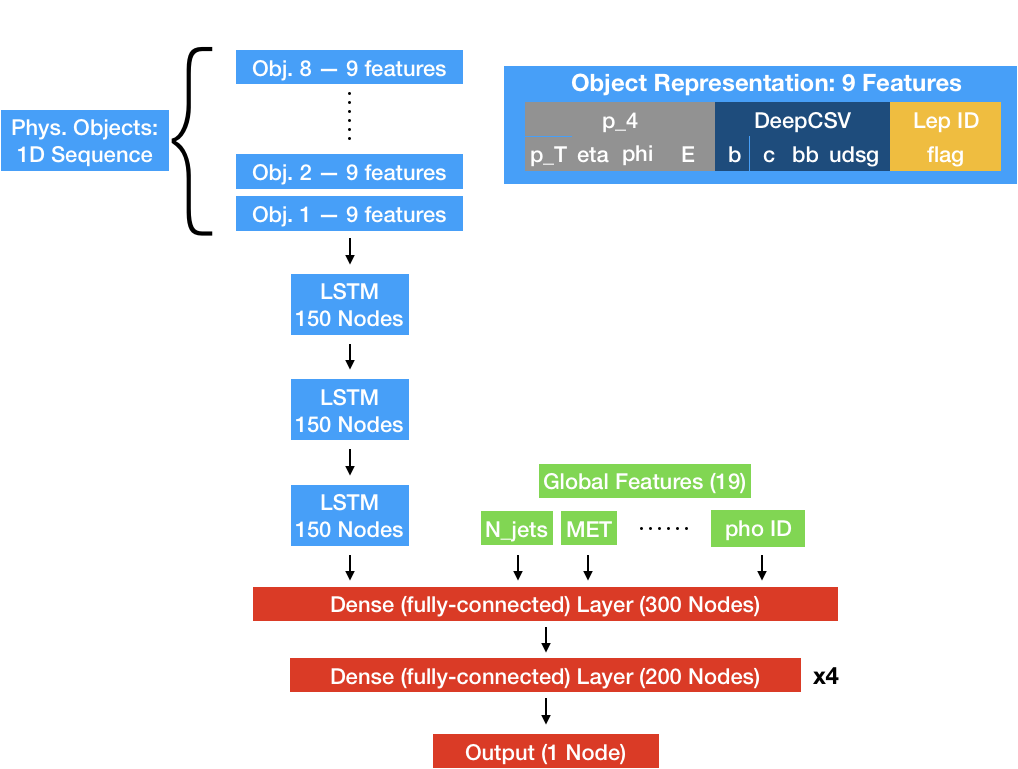
\includegraphics[width=0.7\linewidth]{figures/tth/leptonic_dnn_diagram.png}
    \caption{Schematic of deep neural network architecture, shown for the leptonic channel.}
    \label{fig:tth_dnn_diagram}
\end{figure}

\subsubsection{Training Details}
The DNN is implemented in \texttt{keras}~\cite{keras} with \texttt{tensorflow}~\cite{tensorflow} backend.
It uses the Adam optimizer~\cite{adam} with a learning rate of of $10^{-3}$ and with a binary cross-entropy loss function.
It is trained with an early-stopping procedure in which the batch size is increased over the course of training~\cite{increase_batch}.
Starting with a batch size of 1024, the DNN is trained until the improvement in 1-AUC, as calculated on the validation set, after each epoch is less than 1\%, at which point the batch size is quadrupled.
This procedure is repeated until the batch size exceeds 50,000, at which point it is capped and the training is stopped when the validation AUC ceases to improve.
The batch size is capped due to technical limitations of the GPU: large batch sizes take up a large amount of memory.
DNN hyperparameters are summarized in Table~\ref{tab:tth_dnn_hyperparams}.

\begin{table} [h]
    \centering
    \begin{tabular}{l l}
        Hyperparameter & Value(s) \\ \hline
        Number of nodes (fully connected layers) & 300, 200, 200, 200, 200 \\
        Number of nodes (LSTM layers) & 150, 150, 150 \\
        L2-normalization constraint (``maxnorm'') & 3 \\
        Dropout rate & 0.1 \\
        Learning rate & $10^{-3}$ \\
        Batch momentum & 0.99 \\
        Activation function (LSTM) & hyperbolic tangent \\
        Activation function (fully-connected layers) & exponential linear unit \\
        Activation function (output layer) & sigmoid \\
    \end{tabular}
    \caption{Hyperparameters for the deep neural networks used in both the hadronic and leptonic channels.}
    \label{tab:tth_dnn_hyperparams}
\end{table}

A number of regularization methods are employed, which were found to improve performance and/or convergence speed during training.
First, training features are preprocessed with a `Z-score'' normalization procedure, subtracting the mean and dividing by the standard deviation of each feature such that all features have zero mean and unit variance.
In addition to the Z-score transformation, input features with units of GeV are given in terms of their logarithm, with the log taken before the Z-score transformation.
The aim of preprocessing is to provide a uniform scale for all input features, as this results in faster convergence during training and even improved performance~\cite{lecun_efficient_backprop}.
In the same spirit as feature preprocessing, batch normalization~\cite{ioffe2015batch} is applied between the fully-connected layers of the DNN, normalizing each layer's inputs.
Batch normalization is not applied in between the LSTM layers.
Both feature preprocessing and batch normalization resulted in faster convergence and improved performance of the DNNs.
In addition, dropout~\cite{dropout} is applied between the fully-connected layers in order to reduce overfitting and improve performance.
Between layers which apply both batch normalization and dropout, batch normalization is applied first and dropout is applied second.

\subsubsection{Performance}
Three separate DNNs are trained:
\begin{itemize}
    \item Hadronic channel: \ttH vs. \dipho
    \item Hadronic channel: \ttH vs. \ttgg
    \item Leptonic channel: \ttH vs. \ttgg
\end{itemize}
The output of each DNN is shown for both data and simulation in Fig.~\ref{fig:tth_dnn_datamc}.
\begin{figure} [htbp!]
    \centering
    \begin{tabular}{c c}
        \includegraphics[width=0.48\linewidth,page=58]{{figures/tth/ttHHadronic_RunII_MVA_Presel_v4.11_7Apr2020_impute_histogramsRunIIstd}.pdf} &
        \includegraphics[width=0.48\linewidth,page=59]{{figures/tth/ttHHadronic_RunII_MVA_Presel_v4.11_7Apr2020_impute_histogramsRunIIstd}.pdf} \\
        \includegraphics[width=0.48\linewidth,page=69]{{figures/tth/ttHLeptonic_RunII_MVA_Presel_v4.11_7Apr2020_histogramsRunIIstd}.pdf} &
    \end{tabular}
    \caption{Agreement between data and MC description of background for the various DNNs used as input features to BDT-bkg, for the hadronic channel (top) and the leptonic channel (bottom).}
    \label{fig:tth_dnn_datamc}
\end{figure}
The DNNs are used as inputs to the BDT-bkg, rather than in place of the BDT-bkg because superior performance from DNNs was only observed in the case of a high number of events available for training.
The simulation samples describing \ttH, \dipho, and \ttgg processes each have a high number of individual events ($\geq 10^5$) passing the preselection requirements, so DNNs are trained to distinguish between these processes.
The improvement brought to each channel by the DNNs is shown in Fig.~\ref{fig:tth_dnn_za}.
\begin{figure} [htbp!]
    \centering
    \begin{tabular}{c c}
        \includegraphics[width=0.48\linewidth]{figures/tth/za_comparison_data_Hadronic_DNN_2May2020.pdf} &
        \includegraphics[width=0.48\linewidth]{figures/tth/za_comparison_data_Leptonic_DNN_2May2020.pdf}
    \end{tabular}
    \caption{Expected significance ($Z_A$) shown as a function of the number of \ttH events passing a given cut on BDT-bkg for versions of BDT-bkg trained with (red) and without (black) the DNN scores as training features. Shaded bands show the $\pm 1\sigma$ statistical uncertainty in $Z_A$. The background yield is estimated from events in data in the \mgg sidebands.}
    \label{fig:tth_dnn_za}
\end{figure}
The improvement in expected sensitivity in the hadronic channel is about 10\%.
The improvement in the leptonic channel is significantly smaller than the statistical uncertainty in $Z_A$.
The fact that the improvement is greater in the hadronic channel is likely attributed to the fact that it benefits from the DNN trained against the \dipho background.
Not only is this the largest background in the \ttH hadronic channel signal regions, but the simulation sample has the largest number of events entering the preselection, allowing for aggressive DNN training with lower risk of overfitting.

\subsection{Top Tagger BDT} \label{sec:tth_top_tagger_bdt}
The dominant backgrounds in the hadronic channel at both preselection level and signal region level are the multi-jet, \gjets, and \dipho processes.
An obvious difference between these processes and \ttH is the fact that there are two top (anti-)quarks in the latter, while there are none in the former.
This motivates the use of methods which can identify the presence of top quarks as a tool for further rejecting the multi-jet, \gjets, and \dipho backgrounds.

The chosen method is a top tagger BDT, originally developed in a search for supersymmetric partners of the top quark~\cite{stop_search} and later updated for \ttH.
The BDT is trained using \textsc{xgboost}~\cite{xgboost}.
The BDT takes jet triplets as inputs, with triplets that are matched as coming from a top quark (using generator truth-level information) designated as signal and all other triplets designated as background.
Jets are required to have $p_T > 25$ GeV and $|\eta| < 2.4$.
In addition, the jets are cleaned such that they are not overlapping with leptons.
The truth matching enforces the following additional requirements:
\begin{itemize}
    \item $|m_{jjj} - m_t| < 80$ GeV
    \item All three reco jets are matched to generator-level quarks from a hadronically decaying top ($\Delta R(\text{jet, quark}) < 0.4$).
\end{itemize}
The training features are shown in Table \ref{tab:tth_top_tagger_features}.
\begin{table}
	\centering
	\begin{tabular}{c |c c c c} \hline \hline
		Category & \multicolumn{4}{c}{Features} \\ \hline
		\multirow{3}{*}{Single Jet Quantities} & $p_T$ & mass & & \\
		& DeepCSV b & DeepCSV c vs. light & DeepCSV c vs. b & \\
		& ptD & axis1 & multiplicity & \\ \hline
		\multirow{1}{*}{Di-Jet Quantities} & $\Delta R(\text{j,j})$ & $m_{\text{jj}}$ & & \\
		\multirow{1}{*}{Tri-Jet Quantities} & $\Delta R(\text{b,W})$ & $m_{\text{jjj}}$ & &  \\ \hline \hline
	\end{tabular}
    \caption{Input features used in training the Top Tagger BDT.}
    \label{tab:tth_top_tagger_features}
\end{table}
The training features are defined as follows:
\begin{itemize}
    \item DeepCSV scores: for each jet, three DeepCSV quantities are provided: the b-tag score, and the c-tag score, given in terms of c vs. light and c vs. b.
    \item ptD, axis1, multiplicity: standard quark-gluon discrimination variables. The fragmentation function is defined as $\text{ptD} \equiv \frac{\sqrt{\sum p_{\text{T}_i}^2}}{\sum p_{\text{T}_i}}$, axis1 is the jet shape variable describing the jet's long axis, and multiplicity provides the number of constituents in the jet.
\end{itemize}
The jet in the triplet with the highest DeepCSV b score is labeled as the b-jet, while the other two jets are labeled as $\PW$-jet 1 and 2, with $\pT(\PW_{j1}) > \pT(\PW_{j2})$.

The ouput of the top tagger BDT is shown for both data and simulation in Fig.~\ref{fig:tth_top_tagger_datamc}.
\begin{figure} [htbp!]
    \centering
    \includegraphics[width=0.48\linewidth,page=48]{{figures/tth/ttHHadronic_RunII_MVA_Presel_v4.11_7Apr2020_impute_histogramsRunIIstd}.pdf}
    \caption{Agreement between data and MC description of background for the top tagger BDT score.}
    \label{fig:tth_top_tagger_datamc}
\end{figure}
Similar to the DNN scores, the top tagger BDT is given as an additional training feature to BDT-bkg.
The improvement in expected sensitivity gained by adding the top tagger to BDT-bkg is shown in Fig.~\ref{fig:tth_top_tagger_za} and is about 5\%.
\begin{figure} [htbp!]
    \centering
    \includegraphics[width=0.7\linewidth]{{figures/tth/za_comparison_data_Hadronic_TopTagger_2May2020}.pdf}
    \caption{Expected significance ($Z_A$) shown as a function of the number of \ttH events passing a given cut on BDT-bkg for versions of BDT-bkg trained with (red) and without (black) the DNN scores as training features. Shaded bands show the $\pm 1\sigma$ statistical uncertainty in $Z_A$. The background yield is estimated from events in data in the \mgg sidebands.}
    \label{fig:tth_top_tagger_za}
\end{figure}

\subsection{BDT-bkg}
The final BDT-bkg algorithms for each channel use the high-level features listed in Table~\ref{tab:tth_hlf}, the DNN scores described in Sec.~\ref{sec:tth_dnns}, and the top tagger BDT score described in Sec.~\ref{sec:tth_top_tagger_bdt} as the training features.
The outputs of the BDT-bkg algorithms are shown in Fig.~\ref{fig:tth_bdt-bkg}, where agreement between data and simulation is observed within statistical and systematic uncertainties.
\begin{figure} [htbp!]
    \centering
    \begin{tabular}{c c}
        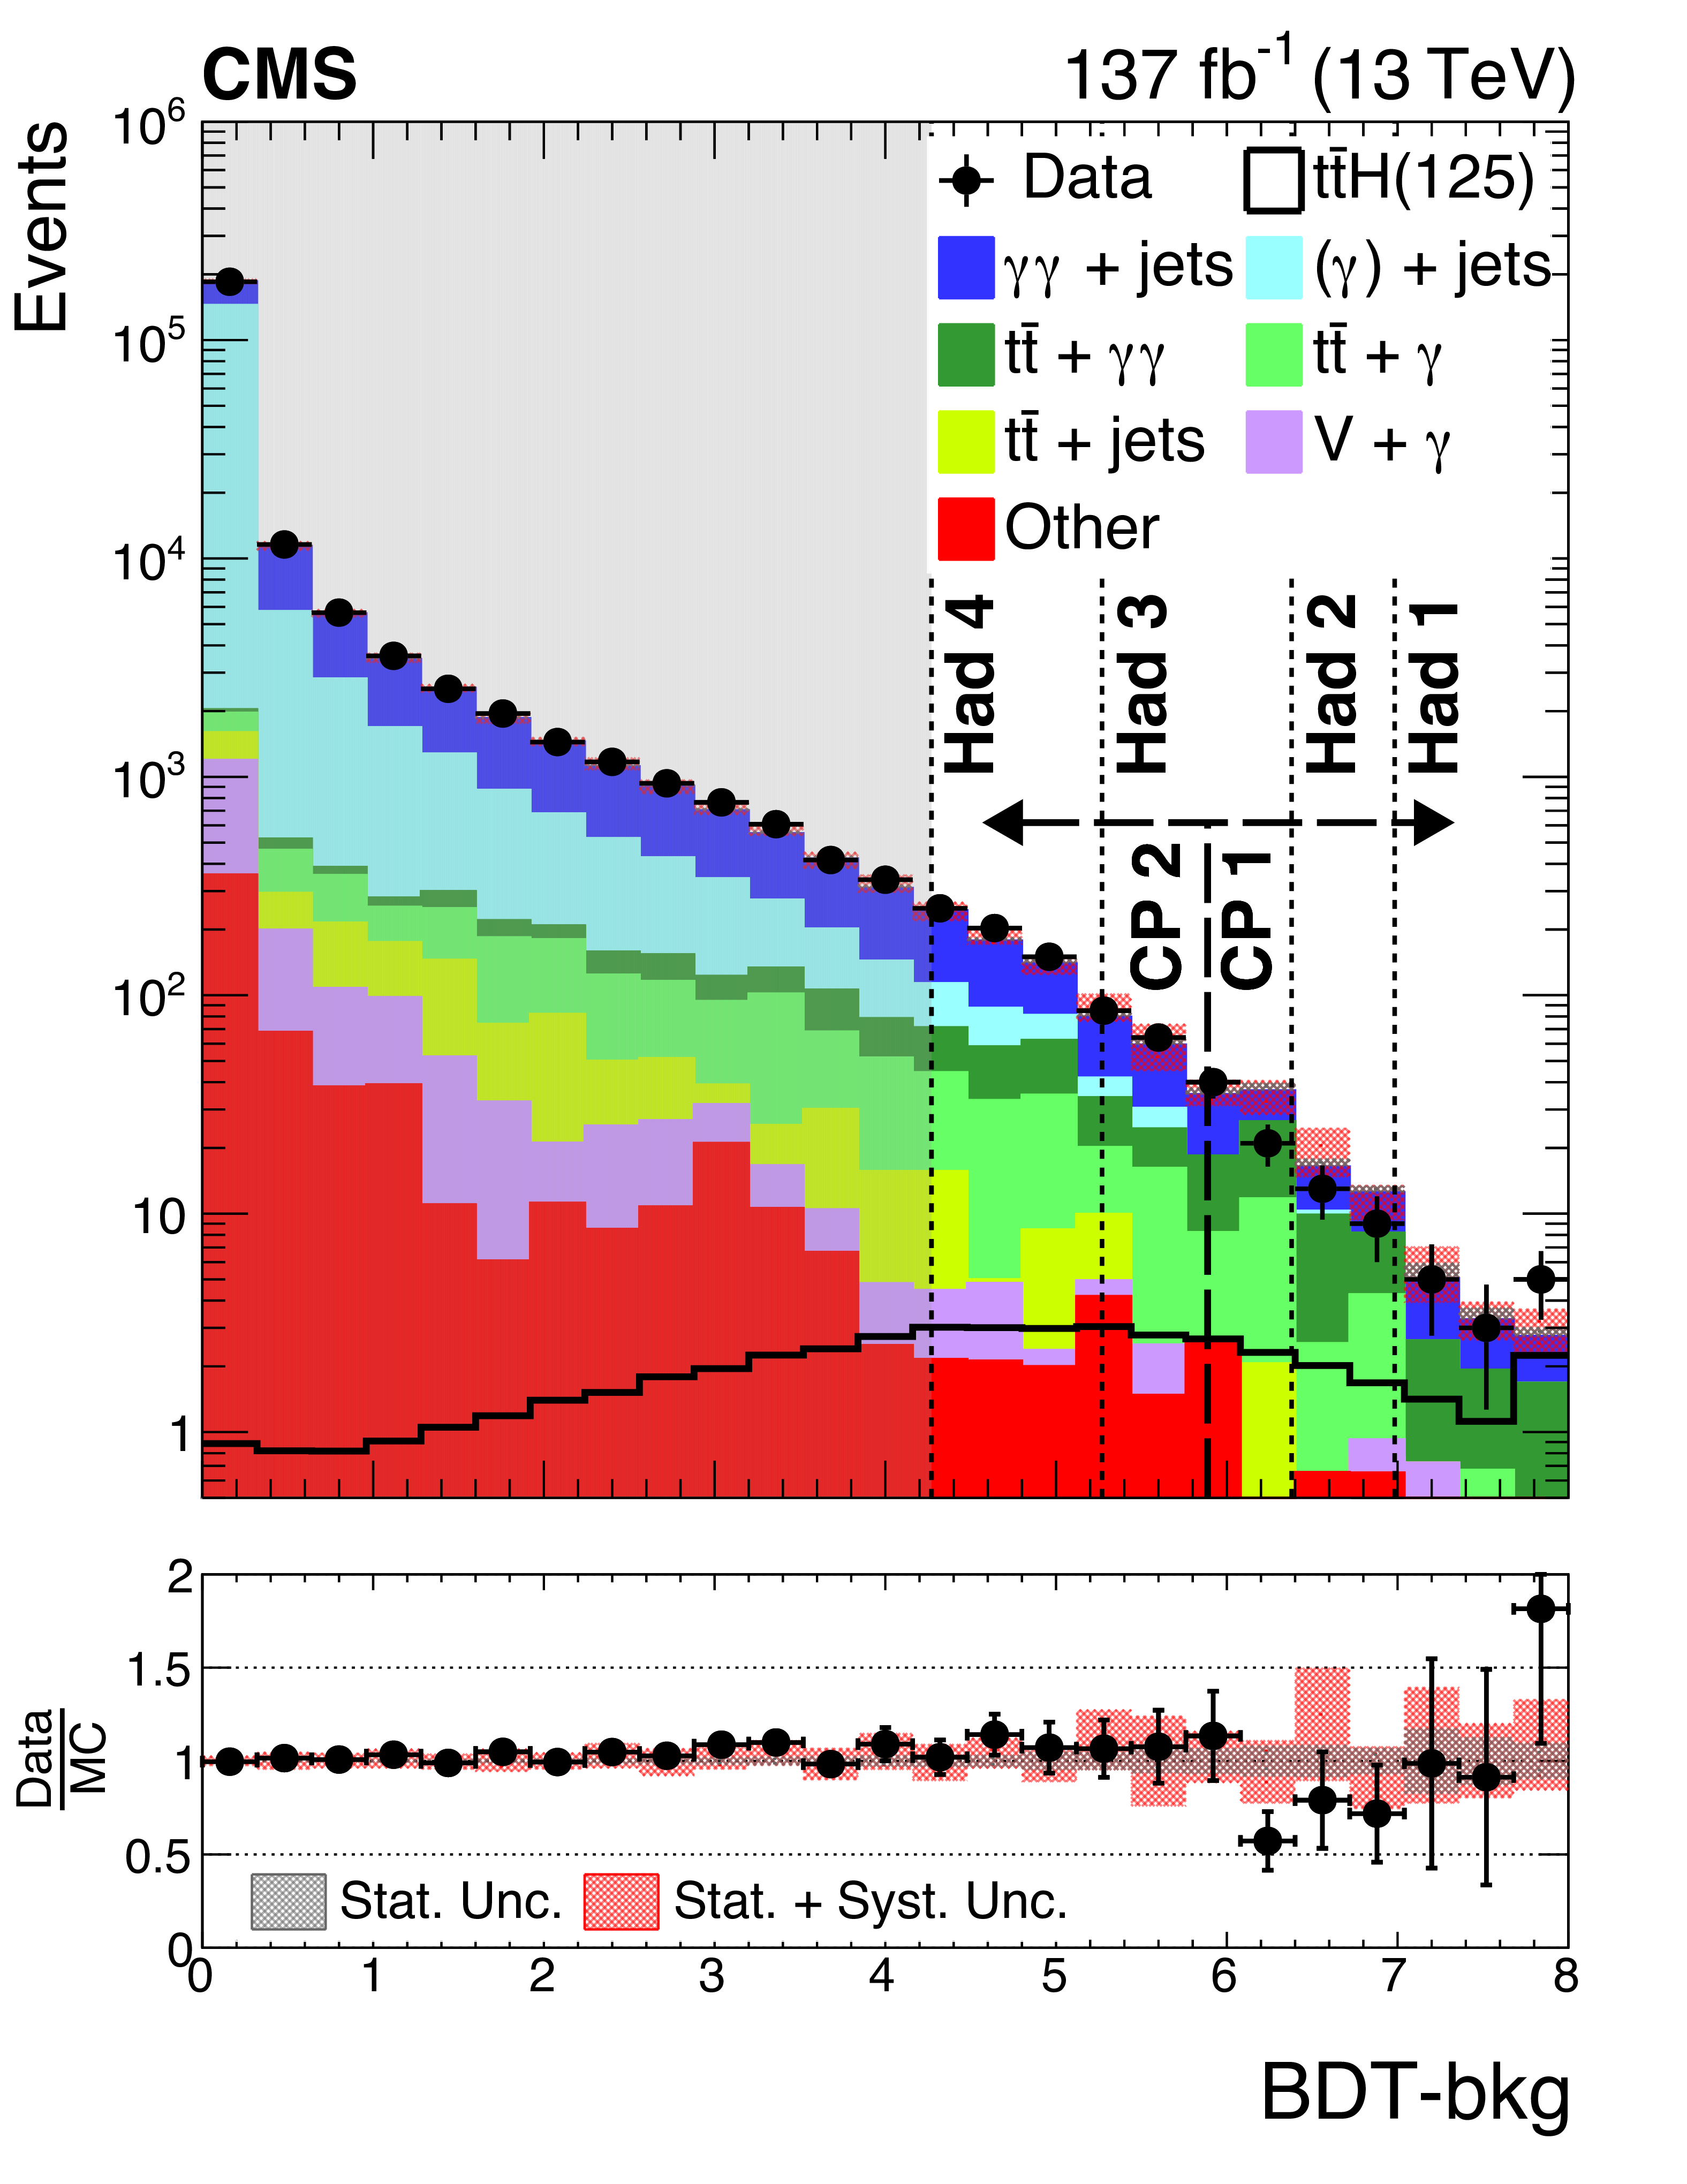
\includegraphics[width=0.48\linewidth]{figures/tth/CMS-HIG-19-013_Figure_001-a.png} &
        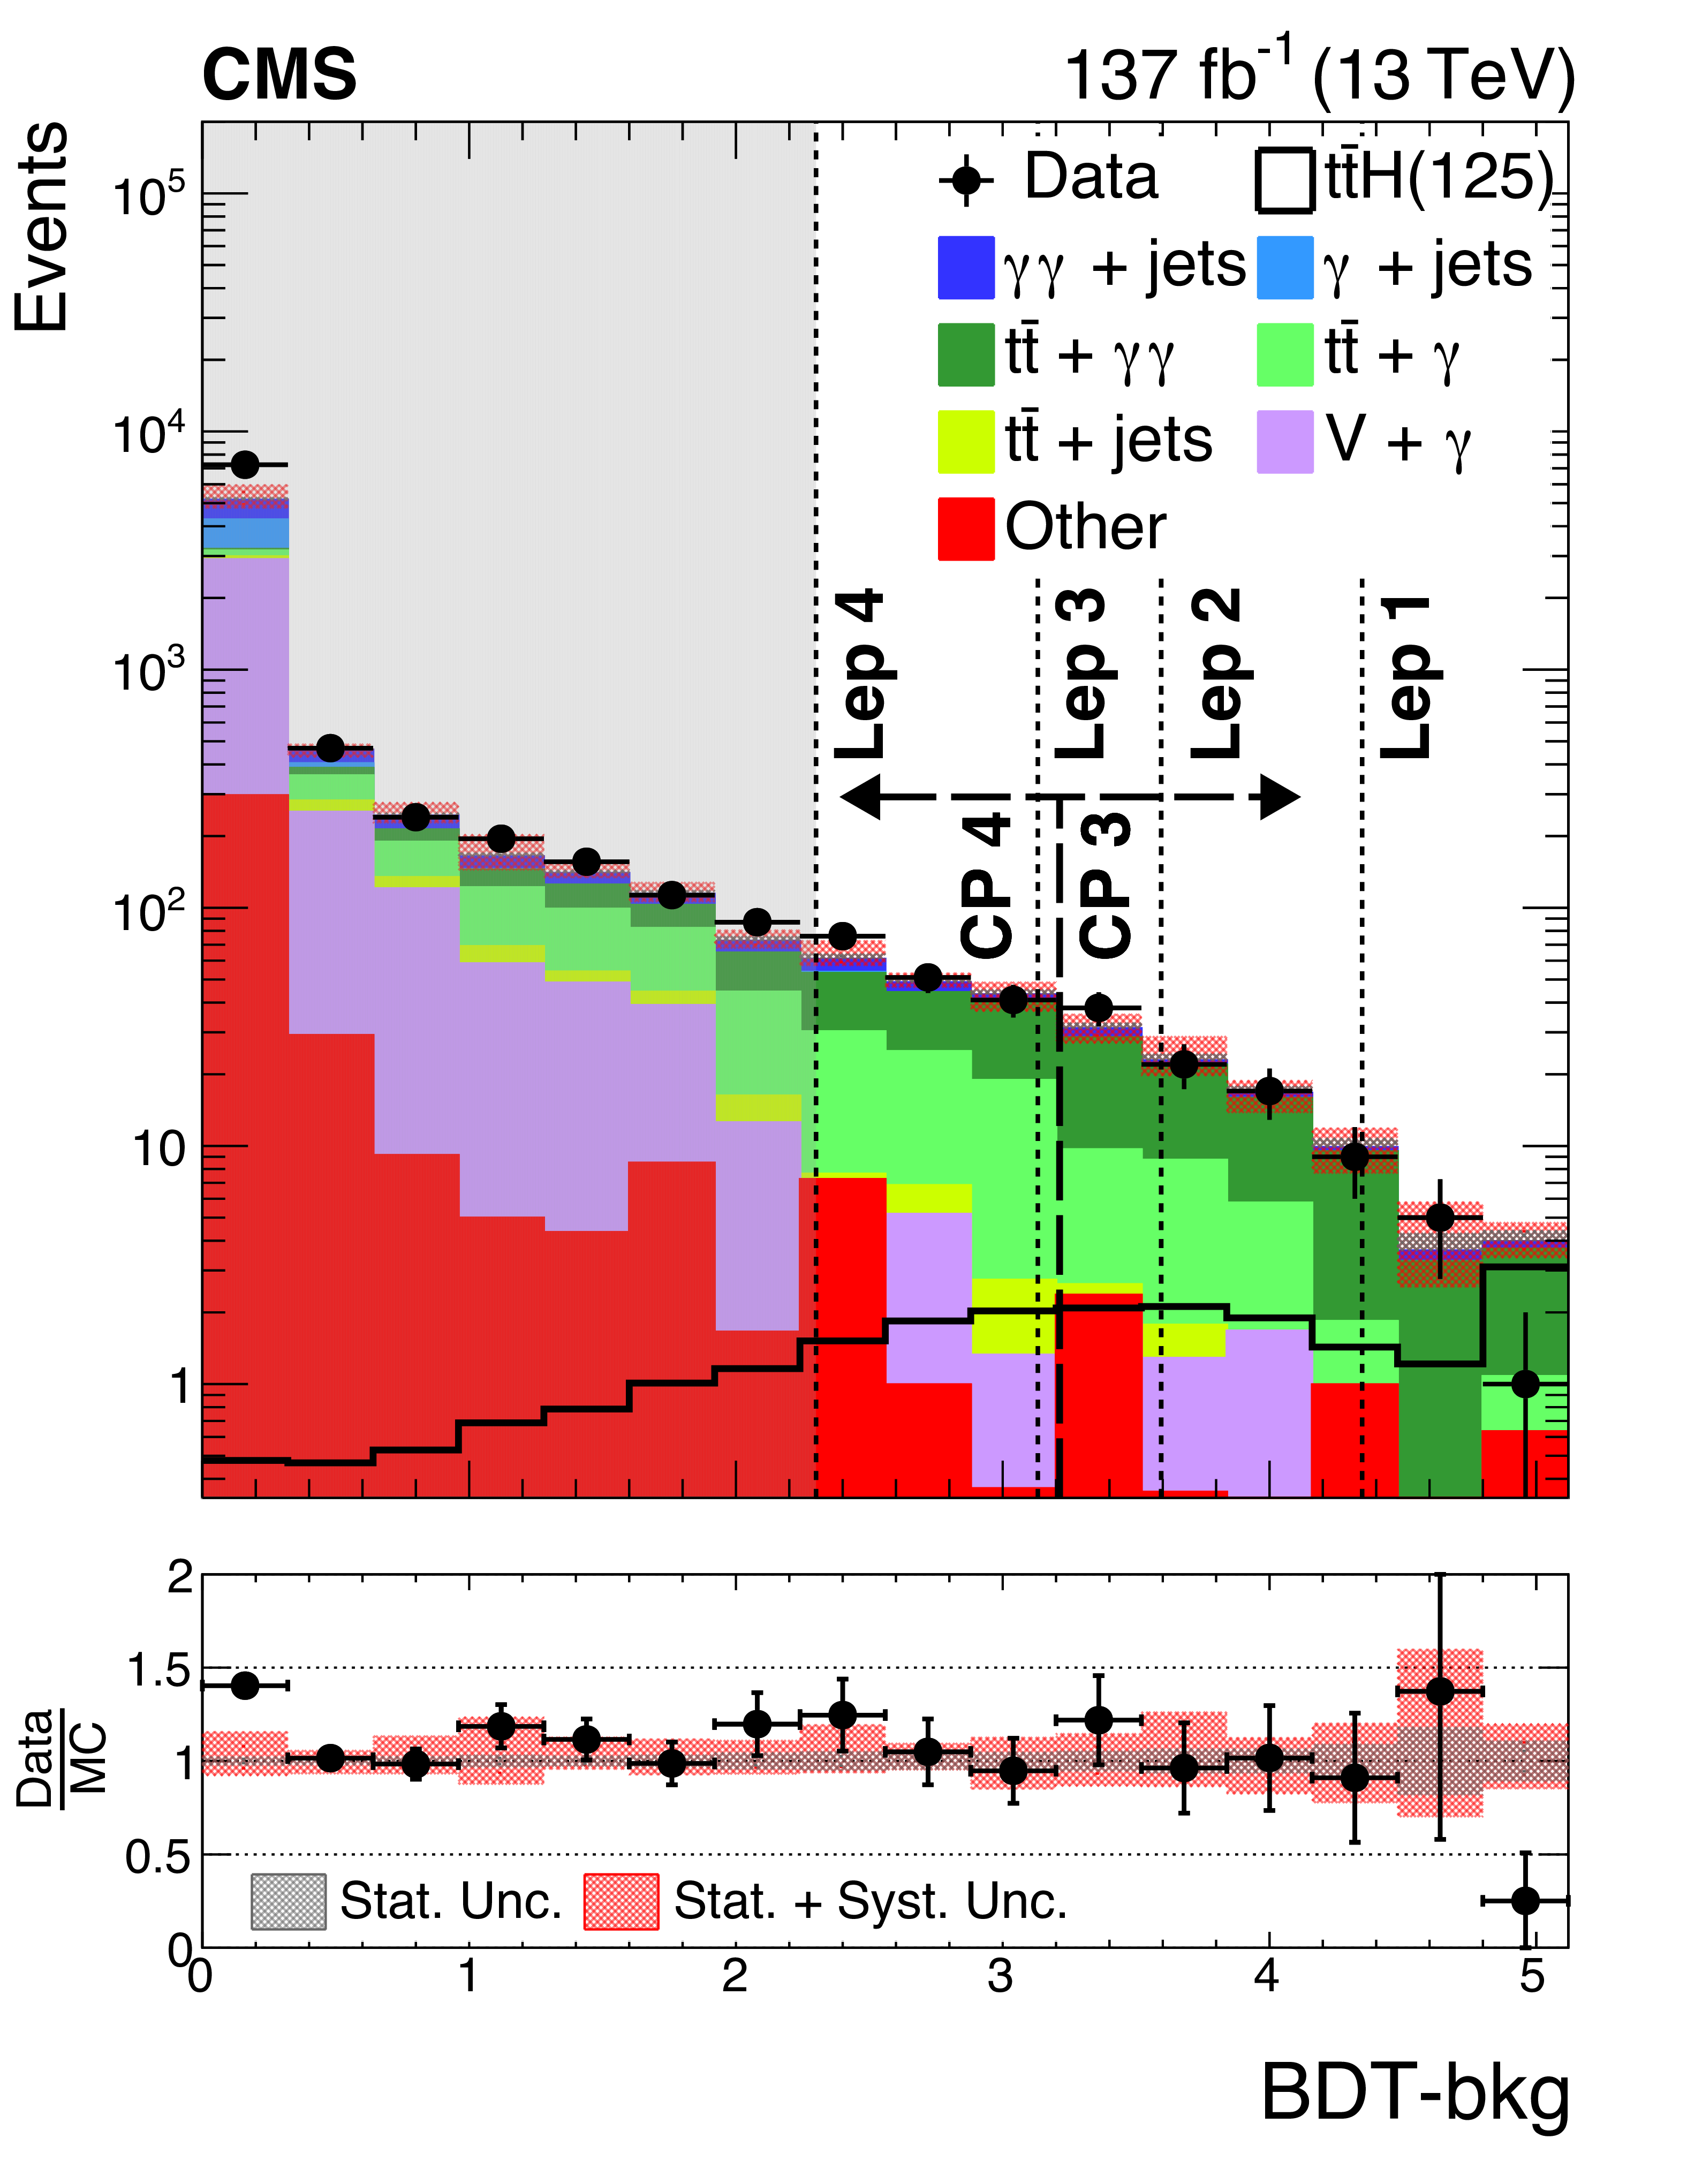
\includegraphics[width=0.48\linewidth]{figures/tth/CMS-HIG-19-013_Figure_001-b.png}
    \end{tabular}
    \caption{Output of the BDT-bkg algorithm for the hadronic channel (left) and the leptonic channel (right). Events from the \mgg sidebands are shown for both data and simulation. The statistical (statistical $\oplus$ systematic) uncertainties in simulation are shown with black (red) shaded bands. The thinly dashed lines show the boundaries of each signal region used for the cross section measurement, while the thickly dashed lines show the boundaries of signal regions used for a measurement of the CP structure. Events in the gray shaded region are discarded.}
    \label{fig:tth_bdt-bkg}
\end{figure}


